%% The following is a directive for TeXShop to indicate the main file
%%!TEX root = diss.tex

\chapter{Introduction}
\label{ch:introduction}
Human beings are physical, social creatures, yet our technology has only just started to communicate on our terms.
Over the years, computing has progressed from symbolic, machine-focused communication like punch cards, assembly languages, and terminal interfaces to physical and natural user interaction.
Despite embracing new interaction techniques like touchscreens and voice control, the rich senses of touch have been relegated to buzzing alerts or limited to high-stakes expert systems like laparoscopic surgery.

Haptic technology involves the senses of touch, both tactile (skin-based) and proprioceptive (force- and position-based) perception.
Between the resurgence of consumer virtual and augmented reality (VR \& AR), rapid development of personal fabrication techniques, and recent additions of high-fidelity haptics to wearable products like the Apple Watch, we are poised to see haptic technology move from niche roles into mainstream adoption.
This diverse field has been active in creating new devices and understanding human perception for decades, but the development of haptic media and design of haptic experiences remain a critical challenge.
Haptic experiences are rich, diverse, multimodal entities which necessitate in-person interaction and have limited infrastructure.
How can we enable creativity with these experiences?
In this dissertation, I study the process of haptic experience design (``HaXD") and establish guidelines for building interactive software systems to support it.
%Through a series of implemented tools, we build pathways for haptic designers.
%This is complemented by both quantitative and qualitative inquiry to understand how haptic designers' experiences and their process.
%Critically, we examine contextual activities that are naturally supported in non-haptic design design, but break down when applied to touch-based interactions: sketching, editing, browsing, and sharing.
%
%
%\section{The state of haptic experience design}
%Haptics is great for many applications.
%Some of the highest profile benefits come from high-resolution medical contexts like remote surgery or dentistry simulation.
%More prevalent, wearables have opened up a wide variety of contexts for unobtrusive tactile feedback, such as exercise bands.
%Accessibility remains an important use for touch-based technology for when other modalities are unavailable.
%Affective display, like communicating the emotions of a loved one, can take advantage of the personal nature of touch.
%%VR \& AR
%
%Of course, lots of work has gone into understanding how to make effective haptics.
%Design guidelines tell us effective ways to communicate large sets of information, provide spatial guidance, and even how to perform tactile concerts.
%% tactile icons and tactons to more sophisticated affective qualities ...
%Several editors and design tools have been built to create
%However, they don't consider the wider context of design: the fact that creativity is a social process that takes place in our environment, where designers build upon new ideas, receive feedback from others, and incroporate their personal experience into their designs.
%
%
%
%
%\section{Creativity in context}
%A painter snatches her paintbrush, sets her easel, and begins.
%An image of \emph{La Grande Jatte} slowly emerges, one stroke at a time, each colour carefully considered.
%What is missing from this scene?
%First, the landscape: is it laid out in front of our painter, referenced from a photograph, remembered, or purely imagined?
%Does she stand alone, or is there a friend giving an impression?
%How does she feel on this particular day, and is she painting for fun or money (or both)?
%
%In this dissertation, I make a simple argument: context must be considered for creative tasks. I then apply this argument to haptic experience design.
%The central goal is arguing for an embodied process of design, a systems model of design. This is applied to both a single haptic experience (consider hardware, user, etc. and all the challenges that this system entails), and to the designer?s process, situated in customers, colleagues, examples, and the design right in front of her.
%
%Many people have argued that creativity is not a solitary endeavor; Mihaly (cite), Warr (cite), shneiderman (...). Buxton, ... .
%Recent design research has empirically evaluated this ... Kellmmer, Dow, Hartmann, ... .
%
%Ultimately, creativie interfaces must have low-bar, wide walls, high ceiling; haptic desogn has none of these.
%
%
%
%\section{The difference of haptics}
%By applying advanced design and creativity thinking to haptics, we find two things: 
%1) a way to further improve haptic design, empowering designers, developers, and end-users to create for this new field, and 
%2) a confirmation and elaboration on design thinking.
%Many ideas that are taken for granted in graphic design break down when applied to haptics. 
%This makes us think more critically about design and creativity, and can inform other fields by showing us how haptic experience design is different, and supporting design processes for other, future technologies that are still emerging. (Examples ???)
%
%
%\section{Approach and Contributions}
%describe methodology - design working tools, study process, design extra toools, design haptics, and talk to designers from ground up.
%Multi-pronged approach to understanding this problem.
%
%List of chapters here:
%
%
%
%\osC{bookmark}
%Haptic sensations enable engaging, personal, and low-attention experiences, but this is limited due to little support for \emph{designing} a haptic sensation.
%Computer-controlled haptic experiences are a recent phenomenon; the focus on technology requirements and rapidly changing field has left little room for examining processes of design in a methodical way.
%

\section{Haptic Experience Design (HaXD)}
We define ``haptic experience design'' (\haxd) as:
\begin{quote}
\it The design (planning, development, and evaluation) of user experiences intentionally involving both interactive technology and one or more perceived senses of touch, possibly as part of a multimodal or multisensory experience.
\end{quote}
%OS 04.21 We need a definition of haptic experience design, either from lit or create our own.
%KM 04.25 clarify relation to multimodal design (this is one of the challenges)
We use \haxd instead of the more general ``haptic design", which can also refer to design practices related to haptics but not directly involving the user experience, e.g., mechanical design of a new actuator or software design of a new control method.
Our definition also includes pseudo-haptics \cite{Pusch2011} and other illusions that trick the user into thinking haptic feedback is occurring without direct tactile or kinesthetic stimulation.
%OS 06.09 should we also include tangibles?
For brevity, we will use ``haptic designers" to refer to haptic \emph{experience} designers.
%In this work, we shed light on \haxd, documenting the challenges that are unique to or accentuated in haptic design, and applying  design thinking to those challenges.



Here, we also take a systems approach to design.
Designers do not exist in a vacuum, but rather in in a physical, social, and cultural context, and are shaped by their personal experiences.
As we will elaborate, diverse activities are involved in design, including \emph{browsing} examples, \emph{sketching}, \emph{refining}, and \emph{sharing}.
Just as a user's physical, social, and cultural context must be considering in an interactive experience, so too must a designer's.


\section{Approach}

While many tools exist to support design in other modalities, such as graphic design, there are few for haptics.
Part of this comes from immaturity of the field and lack of market penetration of highly expressive haptic devices.
However, there are also intrinsic challenges to designing for the sense of touch.
%I want to develop practical tools that support the HaXD process, building a body of knowledge of how to facillitate this difficult subfield of design.
I approach this problem with three different strategies:
\begin{enumerate}
\item \textbf{Depth: Vibrotactile design tool case studies (Chapters \ref{ch:hapticinstrument}-\ref{ch:macaron}).}
To understand design, I take a design perspective.
In each of three case studies, I design, build, and evaluate a tool to support an aspect of haptic experience design, scoped to \emph{vibrotactile} (VT) design.
Each of these results in concrete implications for designing tools and a small window onto the larger HaXD process.
Contributions include algorithms, data structures, interaction techniques, features, analytic techniques, and working software tools that have been employed by designers.
\autoref{ch:hapticinstrument}, \autoref{ch:tactileanimation}, and \autoref{ch:macaron} outline these.

\item \textbf{Breadth: Focused haptic design projects (Chapters \ref{ch:hapturk} and \ref{ch:applications}).}
While the case studies provide an in-depth investigation into vibrotactile sensation design, results may not generalize to other devices, and provide limited investigation into design activities like sharing.
To generalize from vibrotactile effects, explore other aspects of haptic design, and gain personal experience as a haptic experience designer, I participate in several smaller side projects.
These more focused projects lend a broader context to our findings.
\autoref{ch:hapturk} and \autoref{ch:applications} discuss these projects.

\item \textbf{Ground: Data from haptic experience designers (Chapter \ref{ch:hapticianinterviews}).}
Finally, despite the recent growth of the field, haptic designers remain relatively rare and difficult to recruit.
To complement my primarily design-based approach and ground it with haptic experience designers in the field, I draw from other data sources: a workshop held at World Haptics 2015 and interviews with haptic designers.
Described in \autoref{ch:hapticianinterviews}, this synthesized contribution provides additional concreteness to the characterization of haptic experience design.
\end{enumerate}



\begin{figure}[htbp]
\begin{center}
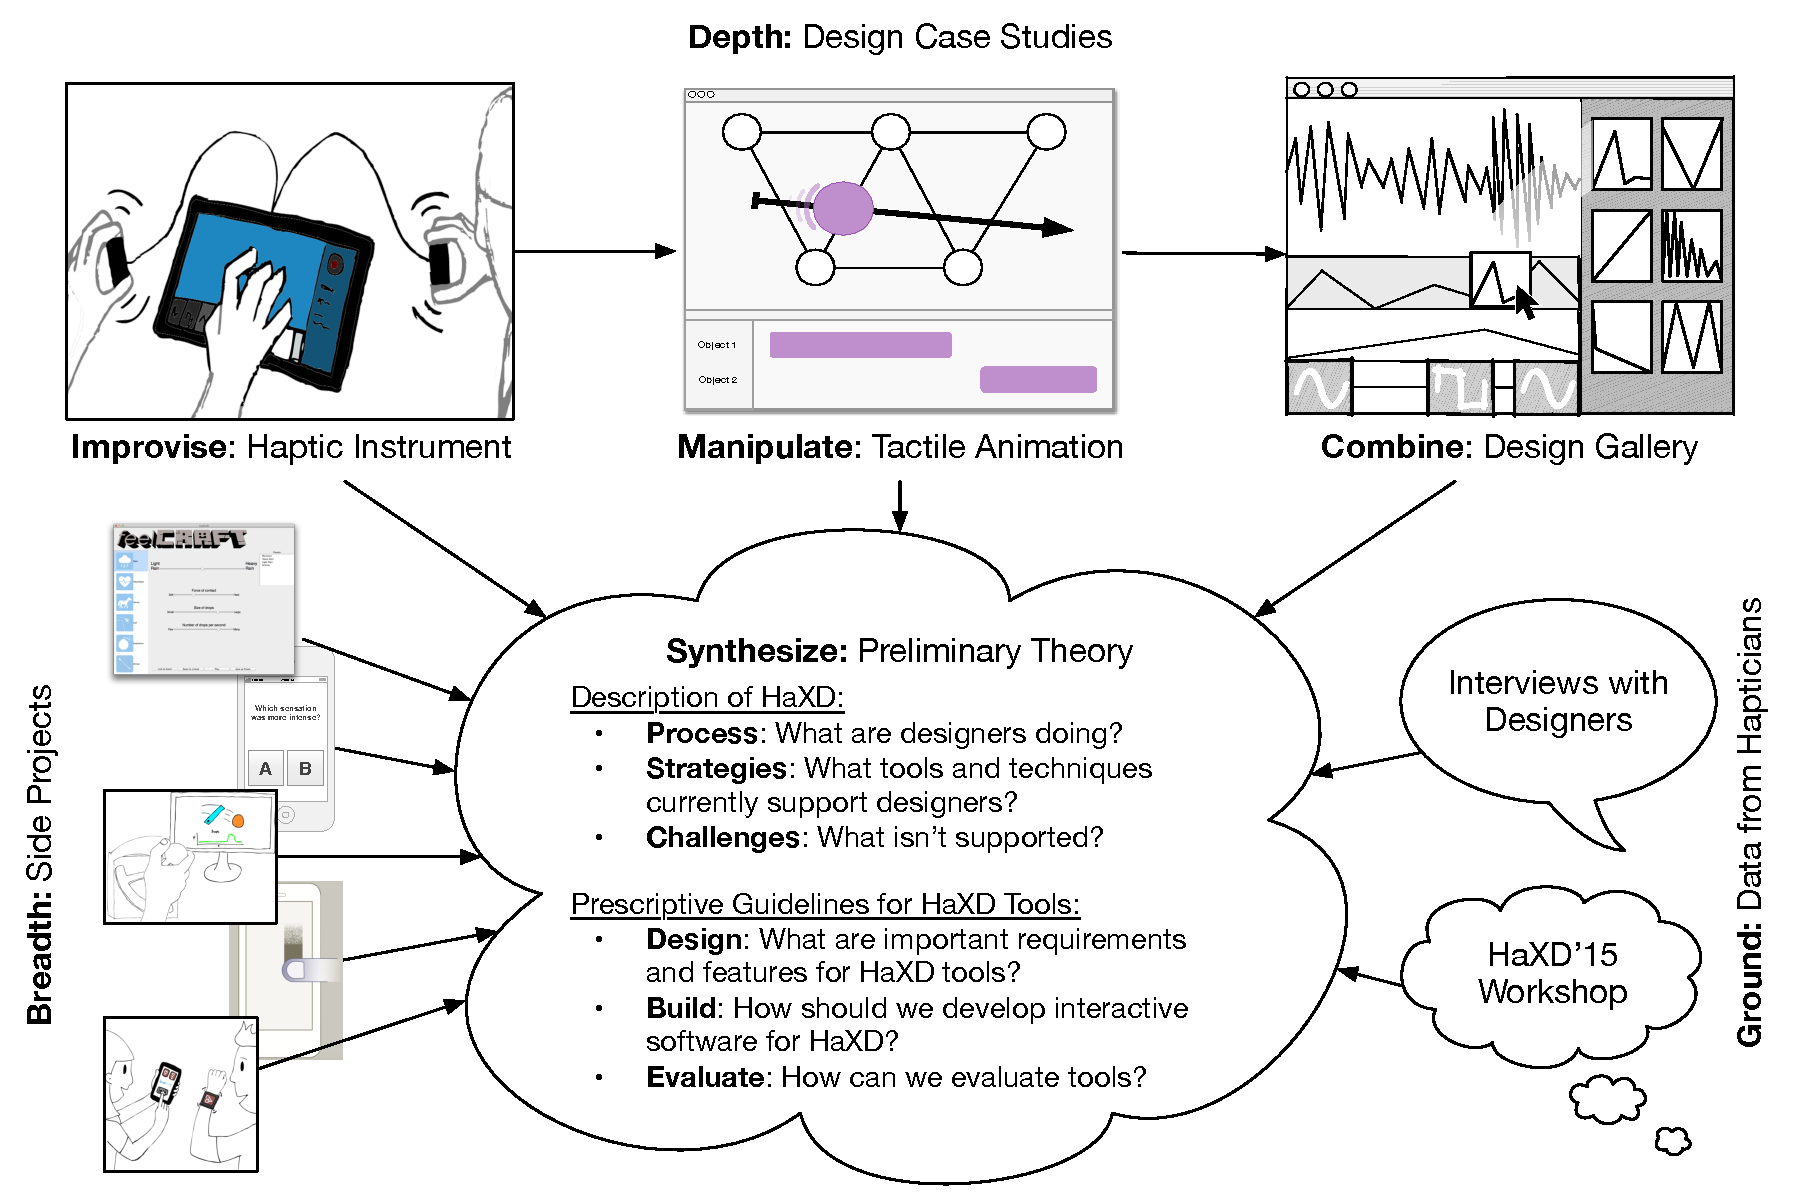
\includegraphics[width=\textwidth]{HaXDTheoryOutline-2015-05-22}
\caption{Approach overview. Three case studies investigate VT tools in-depth; findings are synthesized with side projects and grounded data into a preliminary theory.}
\label{fig:intro:methodologyoverview}
\end{center}
\end{figure}






\subsection{Depth: Vibrotactile Design Tool Case Studies}

Each case study investigates a different set of design concepts with varying user populations, VT device, and design challenges (\autoref{fig:intro:casestudyoverview}), but restricts scope to VT sensations.
This offers a deep look into an expressive and increasingly common class of haptic devices, allowing us to explore critical features in a somewhat controlled fashion.
An iterative approach allows us to refine ideas and methods, and so each case study follows three steps: \emph{gather}, finding requirements and previous design elements; \emph{create}, where we design and build the tool; and \emph{evaluate}, where we test the tool with its target population and consolidate lessons learned.

\begin{description}

\item[Initial Exploration: The Haptic Instrument (\autoref{ch:hapticinstrument})]
In Study 1, the Haptic Instrument, we focus on real-time, rapid design of VT sensations with a first look into themes of real-time design and collaboration.
When participants worked with our tool, mHIVE (a ``mobile Haptic Instrument for Vibrotactile Exploration"), compositions couldn't be edited, suggesting mHIVE was suitable for exploration and improvised communication, but not as suited to refining ideas.
We also found informal, collocated collaboration useful, but leave future examination of collaboration support to side projects (described next in \autoref{ch:intro:approach:breadth}).

\item[Direct Manipulation Pipeline: Tactile Animation (\autoref{ch:tactileanimation})]
In Study 2, Tactile Animation, we developed a single abstracted animation object directly manipulated in both space and time.
In this study, we focused on building a usable tool to support exploration and refinement, and investigate a generalized rendering pipeline in detail to understand how to build haptic design tools.
Animators found our tactile animation tool, Mango, easy-to-use, and confirmed our findings about the value of real-time exploration.
We also found that ``soft features", like copy/paste and undo/redo, were extremely important.

\item[Example Use and Analytics: Macaron (\autoref{ch:macaron})]
One stand-out result from both Mango and mHIVE is that designers drew from their experience or examples found in the world, and wanted to re-use what they had created (e.g., through copy and paste).
In Study 3, we explore the role of examples in haptic design with a web-based tool, ``Macaron", a vibrotactile track-based editor with visible, incorporable examples directly embedded in the interface.
Macaron was implemented using the understanding we gained from Study 2, giving us more opportunity to focus on capturing and studying the design process, especially using interaction logs to investigate example use.
%This study is codenamed ``Project Macaron" and consists of two phases.
%Phase I, ``algorithms and interaction techniques", builds a set of perceptually-verified ways to manipulate examples and incorporate them into designs.
%In Phase II, we use the results of Phase I to create a haptic design gallery interface, and study how and when users incorporate examples into their VT designs.
%In this way we hope to consolidate our findings from mHIVE and Mango, and capture our participants' design process more concretely through logging of user actions.
We found examples were used primarily as templates to inform initial design, making each individual design easier but also scaffolding the user's understanding of how to create VT effects.
%These studies are described in more detail in \autoref{ch:hapticinstrument},  \autoref{ch:tactileanimation}, and \autoref{ch:macaron}.

\end{description}


\begin{figure}[htbp]
\begin{center}
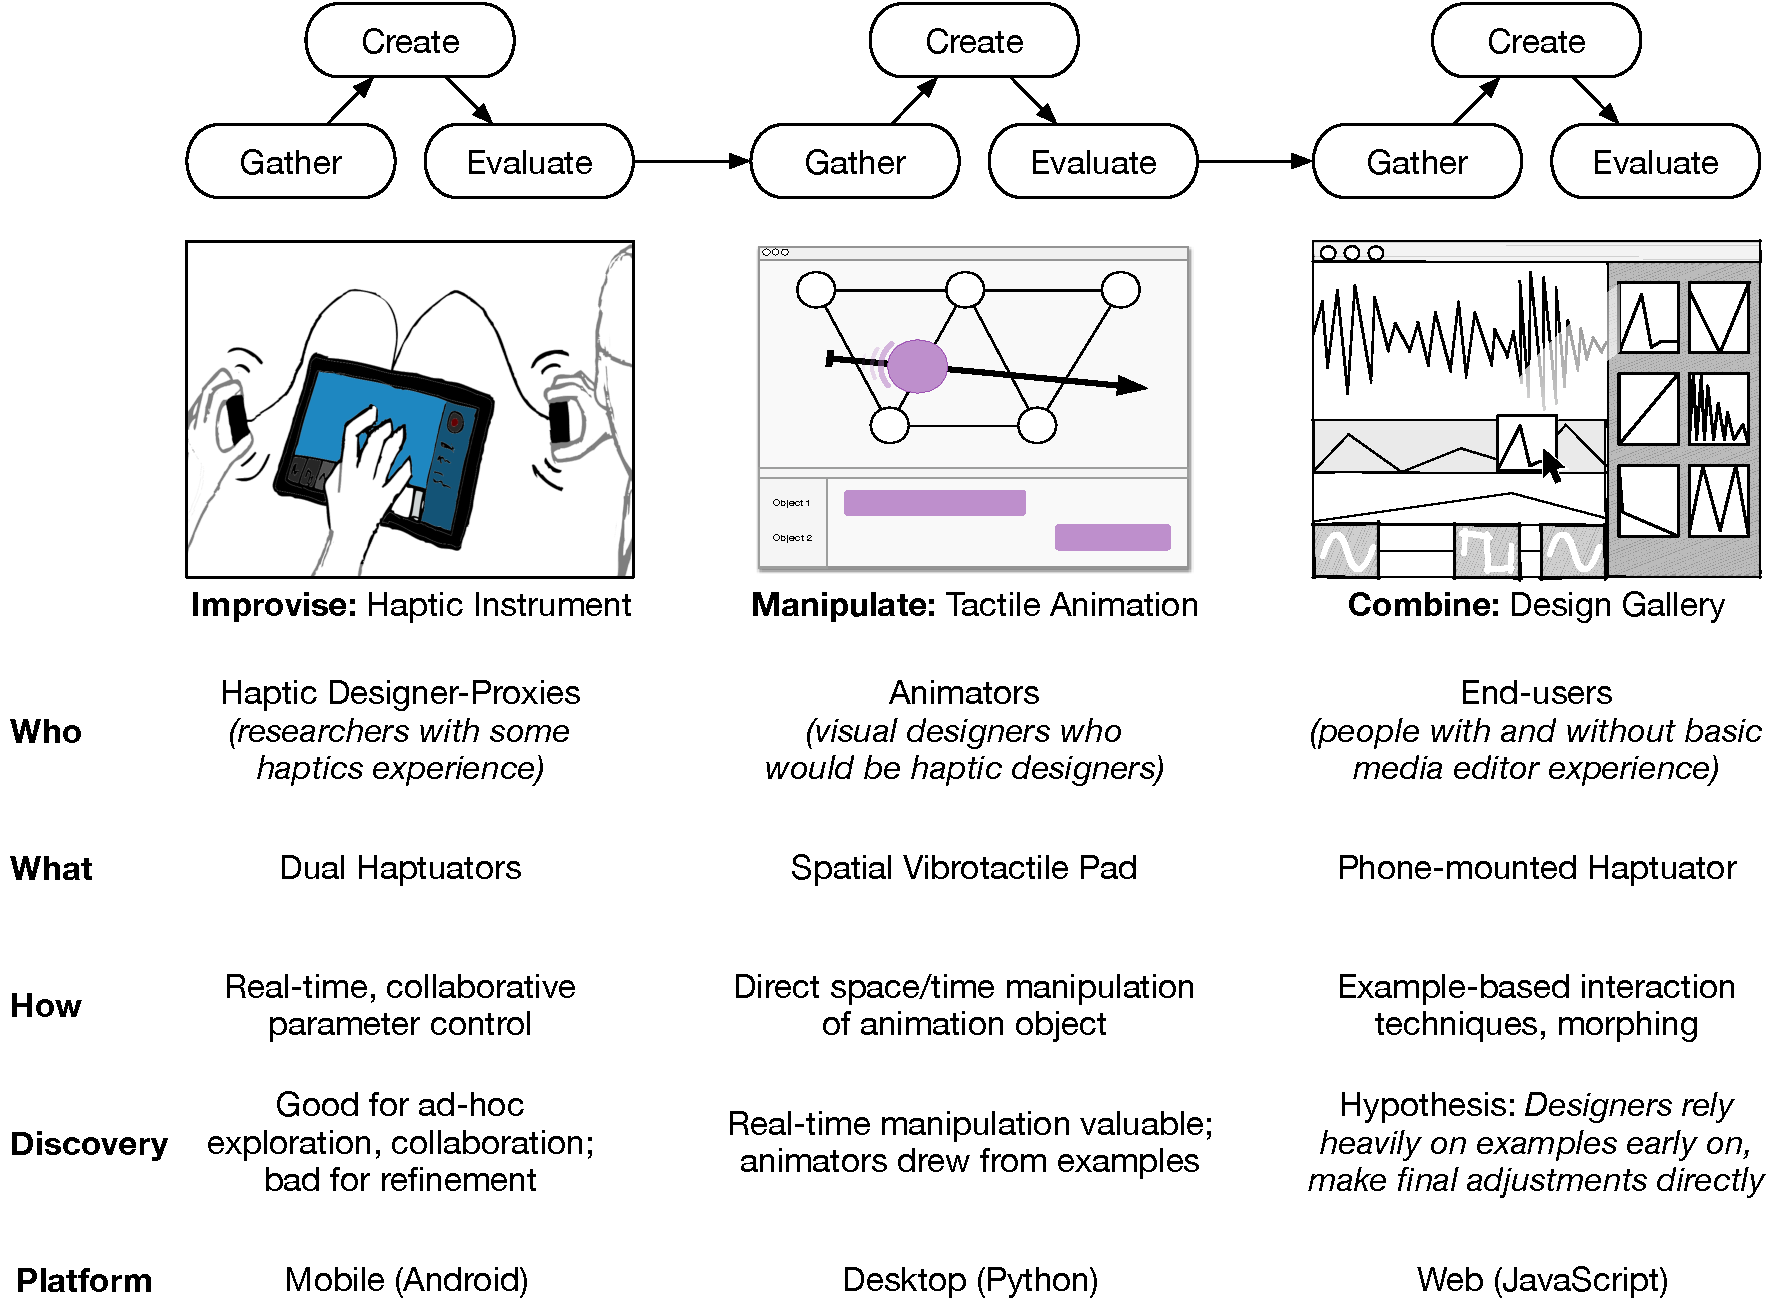
\includegraphics[width=\textwidth]{HaXDTheoryCaseStudyOutline-2015-05-28}
\caption{Vibrotactile design case studies. Each studies an aspect of vibrotactile design with a varied set of users, devices, platforms, and foci.}
\label{fig:intro:casestudyoverview}
\end{center}
\end{figure}


\subsection{Breadth: Focused Haptic Design Projects}
\label{ch:intro:approach:breadth}
Each case study provides concrete knowledge for building a VT authoring tool, and some insight into the VT design process.
However, VT technology can be used in many different scenarios, and there are many devices and experiences that involve other haptic modalities.
To broaden our understanding of haptic design, we undertook several more focused haptic design projects to look at different activities, application areas, and haptic modalities.


In \textbf{\autoref{ch:hapturk}}, we investigate in-depth a technique for large-scale feedback:

\begin{description}
	\item[Feedback at Scale: HapTurk]
	%is a collaboration with PhD candidate Hasti Seifi on different techniques to crowdsource feedback on VT icons. Master's student Salma Kashani and undergraduate Matthew Chun are developing visualizations and low-fidelity VT icons during summer 2015.
	is a technique for collecting large-scale feedback on VT icons.
	Haptic devices cannot be sent to hundreds or thousands of people for feedback, but collecting in-lab feedback can be expensive, and informal feedback from colleagues is limited in scope.
	We investigate whether visual or low-fidelity \emph{proxies} can stand in for high-fidelity VT effects.
\end{description}


In \textbf{\autoref{ch:applications}}, we describe several smaller projects that gave opportunities for practicing haptic design and exploring other types of haptic feedback:

\begin{description}
	\item[FeelCraft (\autoref{sec:applications:feelcraft})] is a plug-in architecture that augments media with customizable spatial VT effects.
	We use FeelCraft to explore existing infrastructure for haptic media, and to design VT effects for a popular video game, MineCraft.
	
	\item[Feel Messenger (\autoref{sec:applications:feelmessenger})] is a chat program augmented with expressive, customizable VT effects using commodity hardware and APIs.
	
	\item[RoughSketch (\autoref{sec:applications:roughsketch})] is a painting application for the TPad Phone, a variable-friction mobile device, for the World Haptics 2015 Student Innovation Challenge. 
	Variable friction is a significant contrast to VT sensations as it is intrinsically connected to input: no sensation can be felt without active movement by the user.
	
	\item[HandsOn (\autoref{sec:applications:handson})] is a conceptual model for creative education software using low-cost, DIY haptic hardware, giving us an understanding of how to work with 1-degree of freedom force feedback and an educational context.

	\item[CuddleBit (\autoref{sec:applications:cuddlebit})] is a project inspired by the Haptic Creature [] and CuddleBot project [].
	We use small, breathing robots to explore the display of emotion, and extend our findings from VT design tools into new tools for this modality: Voodle and MacaronBit.

\end{description}





\subsection{Ground: Data from Haptic Experience Designers}
%In addition, it is difficult to find and recruit haptic designers.
\osC{TODO: Update this once I've gone over Ch8 again}
I will synthesize findings from the three design case studies together with a number of side projects, the design literature, community feedback from a workshop on haptic experience design, and interviews with haptic designers into a preliminary design theory on how to support the creation of engaging, captivating haptic experiences.
I expect to make progress on the following questions:


\begin{description}
    \item[Description of the Haptic Design Process.]
    What are the major \textbf{processes and tasks} conducted by haptic designers?
    What \textbf{strategies} do haptic designers employ, including existing tools?
    What are the \textbf{challenges} haptic designers face?
    
    
    \item[Prescriptive Implications for HaXD Tools.]
    What are major \textbf{requirements} and \textbf{features} for designing HaXD tools?
    What are some considerations when \textbf{implementing} HaXD tools in software?
    How can we \textbf{evaluate} design tools effectively?
\end{description}


\section{Outline and Contributions}
\osC{I've already outlined what I'm talking about. What else can I put here to set up the dissertation?}
\osC{TODO: unite this text with some of the previous descriptions, somehow.}
This dissertation continues as follows.
First, in \autoref{ch:rw}, I cover related work with an overview of haptic technology and applications, a presentation of existing haptic design tools, and a discussion of design theory from other fields.

Then, I outline each VT design tool case study in \autoref{ch:hapticinstrument},  \autoref{ch:tactileanimation}, and \autoref{ch:macaron}.
In \autoref{ch:hapticinstrument}, we present findings from our first vibrotactile design tool, the haptic instrument, which supported easy exploration and informal feedback, but identified a key problem: lack of refinement for designs.
In \autoref{ch:tactileanimation}, we present findings from our second vibrotactile design tool, Mango, which established a generalized pipeline and was able to support both exploration and refinement for expert visual animators; it highlighted reuse as an important next step.
In \autoref{ch:macaron}, we present findings from our third vibrotactile design tool, Macaron, which implemented a browsing interface and analytics system; we found examples played a large part of the design process, and that a web-based tool allowed for easy deployment.

%Each chapter is presented as a direct outline of what will appear in the final dissertation, summarizing either methods and results (\autoref{ch:hapticinstrument} and \autoref{ch:hapticanimation}) or proposed methods and possible results (\autoref{ch:hapticexamples}).
I then describe focused haptic design projects in \autoref{ch:hapturk} and \autoref{ch:applications}, and the results from our grounded data collection in \autoref{ch:hapticianinterviews}.\
In \autoref{ch:hapturk}, we document findings from HapTurk, a technique for getting feedback on vibrotactile designs at scale: from the crowd using proxy vibrations distributed over Mechanical Turk; we also comment on uses for haptic broadcasting.
In \autoref{ch:applications}, we synthesize together findings from our side projects, showing generality by applying our understanding of haptic design explicitly in several domains and gaining practical experience designing haptic experience.
In \autoref{ch:hapticianinterviews}, we complement our design-based inquiry through interviews with professional haptic designers and a workshop run to elicit feedback from the community; this captures a description of haptic design, reinforcing our findings for important support tools, and identifies more systematic challenges.

Finally, in \autoref{ch:conclusion}, we conclude with a summary of our final results and directions for future research.


%
% END
%
\endinput

Any text after an \endinput is ignored.
You could put scraps here or things in progress.
